\section{Background and Problem Definiton}
\label{sec:background}

Numerous studies exist on content indexing, with solutions being either centralized or distributed (see Section\ref{related_work}). As explained above, in this paper we advocate designs that do not rely on requesting any remote entity before being able to access a given content.
This section thus focuses on the existing solutions so that: \textbf{for any content, every node is able to access its closest replica without any prior request.}
We explain why existing implementations are costly thus preventing their deployment in real systems.
Then, we describe the problem tackled by this paper at an abstract level to underline the challenges that drove the design of our proposal. 


\subsection*{Disseminate localization information}
Enabling the accessibility of content without prior requests implies that the information about replica localization has to be pushed directly to the nodes.
Broadcasting information about cache updates to all nodes in the system is a straightforward way to maintain consistent information about replica localization for all nodes~\cite{nlsr,lscr}. Indeed, having the entire knowledge of all the replica localizations along with distance information carried into messages, each node can easily compute where the closest copy of a given object resides, without contacting any remote node. Moreover, removing the lookup latency directly involves faster downloading times. 
Similarly, one could solve this issue by using a conflict-free replicated datatype (CRDT) for set data structures, for example~\cite{shapiro2011crdts}. 
However, either by broadcasting or with CRDTs, both inherently imply that every nodes will eventually receive all messages. 
That means information that might only interests a small subset of nodes is actually spread out all over the network. 


\begin{figure}[t]
\centering
\subfloat[Initial configuration - Every nodes get the content from node $R$\label{fig:1a}]{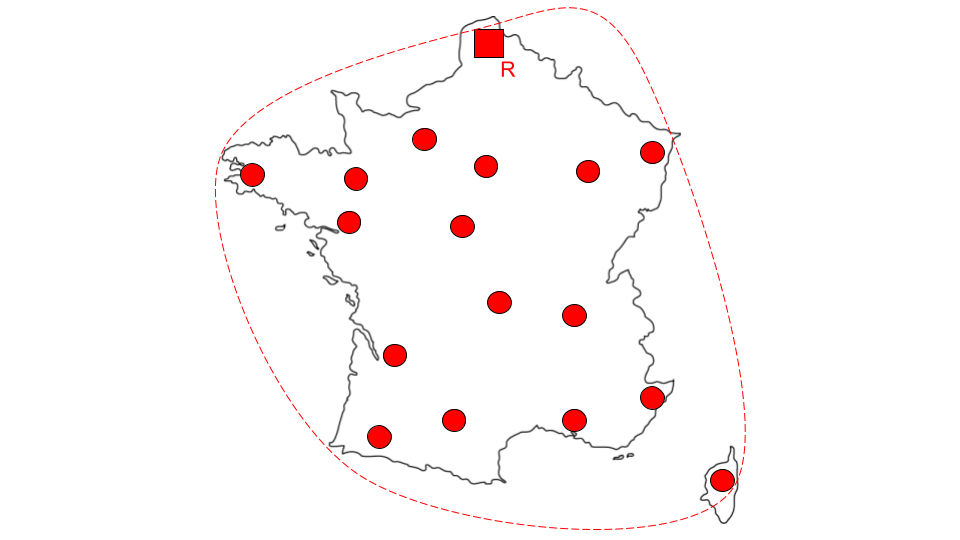
\includegraphics[trim=6cm 0.33cm 6cm 0.33cm, clip, width=0.24\textwidth]{img/Dynamic-partitioning-1.png}}\hfill
\subfloat[Adding a second replica in node $G$ partitions the network nodes in $2$ sets.\label{fig:1b}]{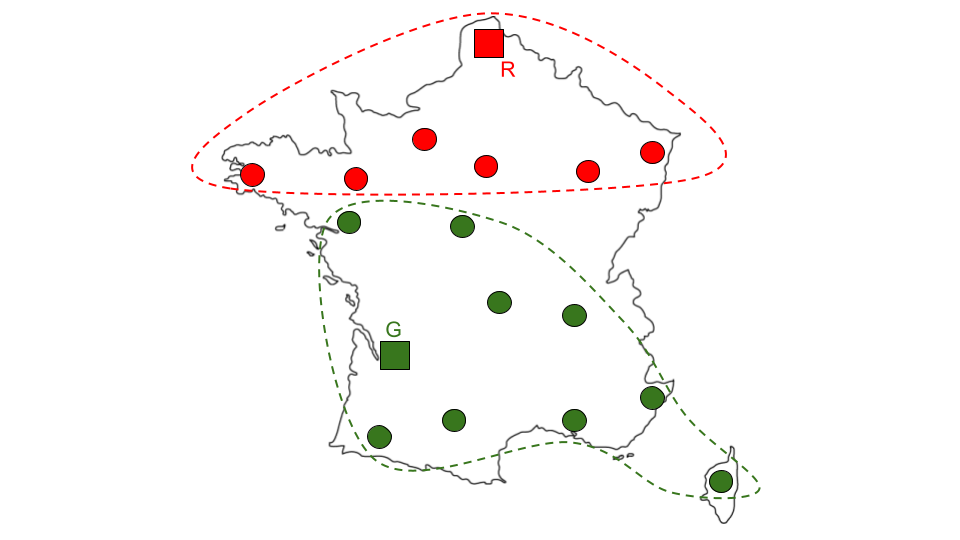
\includegraphics[trim=6cm 0.33cm 6cm 0.33cm, clip, width=0.24\textwidth]{img/Dynamic-partitioning-2.png}}\hfill
\subfloat[A third replica is created in node $B$ resulting in $3$ partitions.\label{fig:1c}]{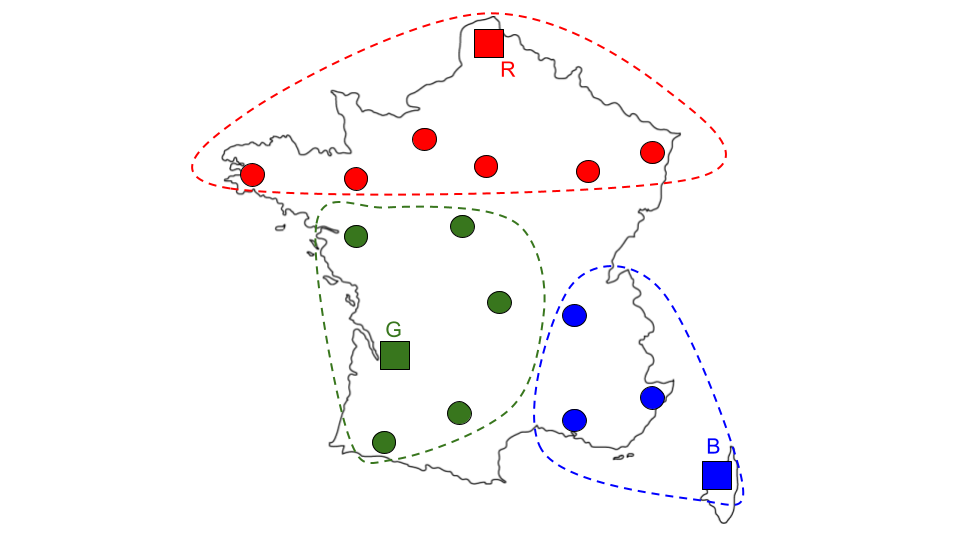
\includegraphics[trim=6cm 0.33cm 6cm 0.33cm, clip, width=0.24\textwidth]{img/Dynamic-partitioning-3.png}}\hfill
\subfloat[Removing the green partition: only $2$ partitions remain.\label{fig:1d}]{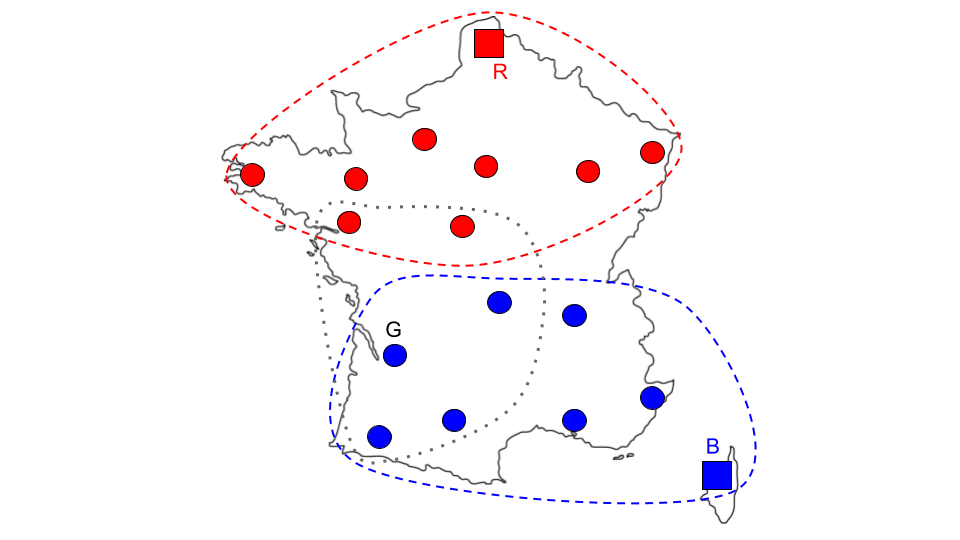
\includegraphics[trim=6cm 0.33cm 6cm 0.33cm, clip, width=0.24\textwidth]{img/Dynamic-partitioning-4.png}}
\caption{Example of the french RENATER topology (edges are not drawn): Partitions shrink or expand according to the creation or removal of replicas. Ideally, only a subset of nodes should be informed of these events, according to their place in the topology.} \label{fig:partition_intuition}
\end{figure}

\subsection*{Locking down the dissemination}
To provide the intuition underlying our proposal, we now describe the problem tackled by this paper at an abstract level, and explain how an (imaginary) omniscient entity could solve it. 
In this way, suppose there exists an \textit{oracle} in the system that instantly knows the arrival/departure of nodes in the topology and the location of the creation/removal of replicas. In other words, this oracle is constantly aware of the current topology and the current list of all available replicas of a given content in the system. Equipped with these two information, it is then trivial for this oracle to compute for each node, where resides its closest replica for a given content. Mapping each node of the topology to a single replica amounts to partition the set of all nodes into $k$ disjoint sets (or partitions), where $k$ is the number of current replicas. Thus, every node in the same partition would get the content from the same replica. Interestingly, this partitioning matches the physical topology as neighbors physically closed in the infrastructure will most likely reside in the same partition.
For any event such as an arrival/departure of nodes or creation/removal of replicas, the oracle is thus able to inform the \textit{exact} subset of nodes that has to update their location (\ie the exact scope of an event). 


This is illustrated in Figure~\ref{fig:partition_intuition} where we depict the partitions shrinking or expanding according to the creation or removal of replicas respectively.
In Figure\ref{fig:1a}, there exists a single occurence of a given content in node $R$: all nodes thus belong to the same partition as they would all retrieve the content from the same node. 
A second replica is created in node $G$ in Figure~\ref{fig:1b}, resulting in $2$ partitions. Nodes from the \textit{green} partition would all obtain the content from node $G$ as it is their closest replica, while nodes from the \textit{red} partition would get it from node $R$.
Note that only the nodes in the green partition has to be informed of the creation of the replica in node $G$. Similarly, in Figure~\ref{fig:1c}, only nodes in the blue partition should be informed of the creation of a new replica in node $B$ as it does not impact other nodes.
Finally, when the replica in node $G$ is removed, nodes in the stale green partition have to join existing ones as illustrated in Figure~\ref{fig:1d}. 
The challenge of implementing such a partitioning in an asynchronous network resides in informing this minimal subset of nodes (or as close as possible), without any \textit{a priori} knowledge while only relying on local information (\ie no node has the knowledge of all the replica localizations).


Finally, we emphasize that information about a given replica localization should remain in a given geographical scope. 
Intuitively, it is most likely that events happening at a given place in the network will have no impact on nodes that are very far away from them.
This prevents the use of gossip protocols for example.  Indeed, gossip protocols are also appealing candidates to disseminate information reliably across a network~\cite{epidemic-protocol} and numerous studies have shown how quickly they converge despite high level of churn and/or failures~\cite{lpbcast}.
However, these protocols usually relies on a so-called \textit{peer-sampling service}~\cite{jelasity2007gossip} to efficiently propagate the information. This implies that nodes will exchange messages with random nodes in the system far exceeding their geograhical scope. 


